\documentclass[11pt]{article}
\usepackage[margin=1.1in]{geometry}
\usepackage{graphicx}
\usepackage{booktabs}
\usepackage{amsmath}
\usepackage{lmodern}
\usepackage{microtype}
\usepackage{caption}
\usepackage{pgfplots}
\pgfplotsset{compat=1.18}
\usepackage[hidelinks]{hyperref}
\usepackage{url}
\captionsetup{font=small, labelfont=bf}

\newcommand{\nTest}{978}
\newcommand{\nDev}{419}
\newcommand{\oracleWer}{2.5}
\newcommand{\truthInList}{89}
\newcommand{\nLists}{1397}
\newcommand{\werNone}{8.1}
\newcommand{\accNone}{69.9}
\newcommand{\werOpt}{7.8}
\newcommand{\accOpt}{71.6}
\newcommand{\tflopOpt}{1.49}
\newcommand{\parOpt}{6700M}
\newcommand{\werQwen}{7.8}
\newcommand{\accQwen}{70.9}
\newcommand{\tflopQwen}{1.69}
\newcommand{\parQwen}{7600M}
\newcommand{\werGpt}{7.8}
\newcommand{\accGpt}{71.3}
\newcommand{\tflopGpt}{0.17}
\newcommand{\parGpt}{774M}
\newcommand{\werGptMed}{7.9}
\newcommand{\accGptMed}{70.7}
\newcommand{\tflopGptMed}{0.08}
\newcommand{\parGptMed}{355M}
\newcommand{\werGptSmall}{8.0}
\newcommand{\accGptSmall}{70.8}
\newcommand{\tflopGptSmall}{0.03}
\newcommand{\parGptSmall}{124M}
\newcommand{\werDistil}{8.1}
\newcommand{\accDistil}{69.5}
\newcommand{\tflopDistil}{0.02}
\newcommand{\parDistil}{82M}
\newcommand{\werJev}{7.5}
\newcommand{\accJev}{71.3}
\newcommand{\werLaya}{8.1}
\newcommand{\accLaya}{69.9}
\newcommand{\tflopLaya}{0.13}
\newcommand{\parLaya}{421M}
\newcommand{\werOptTyped}{8.1}
\newcommand{\accOptTyped}{69.9}
\newcommand{\tflopOptTyped}{2.56}
\newcommand{\parOptTyped}{6700M}
\newcommand{\werQwenTyped}{8.1}
\newcommand{\accQwenTyped}{70.0}
\newcommand{\tflopQwenTyped}{3.24}
\newcommand{\parQwenTyped}{7600M}
\newcommand{\labJev}{57}
\newcommand{\truthPickJev}{67.9}
\newcommand{\labLaya}{44}
\newcommand{\truthPickLaya}{53.7}
\newcommand{\labOptchoice}{13}
\newcommand{\truthPickOptchoice}{27.3}
\newcommand{\labQwenchoice}{31}
\newcommand{\truthPickQwenchoice}{29.3}
\newcommand{\firstPassTopOne}{68.0}
\newcommand{\riskJevAtThirty}{3}
\newcommand{\riskJevAtFifty}{8}
\newcommand{\riskJevAtSeventy}{13}
\newcommand{\riskJevAtNinety}{22}
\newcommand{\riskJevAtHundred}{29}
\newcommand{\riskOptAtThirty}{8}
\newcommand{\riskOptAtFifty}{10}
\newcommand{\riskOptAtSeventy}{17}
\newcommand{\riskOptAtNinety}{24}
\newcommand{\riskOptAtHundred}{28}
\newcommand{\riskGpttwoAtThirty}{9}
\newcommand{\riskGpttwoAtFifty}{13}
\newcommand{\riskGpttwoAtSeventy}{18}
\newcommand{\riskGpttwoAtNinety}{25}
\newcommand{\riskGpttwoAtHundred}{29}
\newcommand{\tokPerCand}{343}
\newcommand{\tokTypedOpt}{191}
\newcommand{\tokTypedQwen}{213}
\newcommand{\qwenTypedAtFive}{76.1}
\newcommand{\qwenTypedAtSixty}{1.5}
\newcommand{\optTypedAtSixty}{55.1}
\newcommand{\baseAtFive}{80.5}
\newcommand{\baseAtSixty}{68.2}
\newcommand{\qwenBorda}{56.9}
\newcommand{\optBorda}{2.7}
\newcommand{\werNoneWeak}{14.1}
\newcommand{\werOptWeak}{10.9}
\newcommand{\werDistilWeak}{12.9}
\newcommand{\oracleWerWeak}{7.3}
\newcommand{\truthInListWeak}{67}
% --- revision additions: combination, sweep, truth-in-list, error analysis ---
\newcommand{\mwerMulti}{7.68}
\newcommand{\mwerMultiP}{0.161}
\newcommand{\gainWeak}{6.8}
\newcommand{\gainStrong}{0.3}
\newcommand{\fpWeakSweep}{19.7}
\newcommand{\nInList}{874}
\newcommand{\nOutList}{104}
\newcommand{\optInListWer}{4.1}
\newcommand{\optInListDelta}{-0.31}
\newcommand{\optInListP}{0.035}
\newcommand{\jevInListWer}{3.8}
\newcommand{\jevInListDelta}{-0.57}
\newcommand{\jevInListP}{0.015}
\newcommand{\subsNone}{7.52}
\newcommand{\subsOpt}{7.20}
\newcommand{\subsJev}{6.63}
\newcommand{\insNone}{0.21}
\newcommand{\insOpt}{0.29}
\newcommand{\insJev}{0.41}
\newcommand{\delsNone}{0.35}
\newcommand{\delsOpt}{0.31}
\newcommand{\delsJev}{0.41}
\newcommand{\nOverride}{94}
\newcommand{\marginR}{0.12}
% --- MWER fine-tuning of GPT-2 small (round 4, GPU) ---
\newcommand{\mwerSmallWer}{8.2}
\newcommand{\mwerSmallDev}{8.0}
\newcommand{\mwerSmallAlpha}{0.5}
\newcommand{\mwerSmallPNone}{0.62}
\newcommand{\mwerSmallPGpt}{0.84}
% Joint re-tuning of the decoder's acoustic weight with alpha (dev only), test split
\newcommand{\werOptJoint}{7.2}
\newcommand{\werQwenJoint}{7.4}
\newcommand{\werJevJoint}{6.9}
\newcommand{\gainOptJoint}{0.9}
\newcommand{\gainQwenJoint}{0.7}
\newcommand{\gainJevJoint}{1.2}


\title{\bf How Much Language Model Does a Speech Neuroprosthesis Need?\\
\large The stronger the decoder, the less rescoring helps}

\author{Gabriele Cin\`a\\\small\texttt{c.gabriele.info@gmail.com}}
\date{}

\begin{document}
\maketitle

\begin{abstract}
\noindent
A speech neuroprosthesis decodes attempted speech from brain activity, and every
high-performance system ends by rescoring the decoder's candidate sentences with a
language model. That stage is the only one that needs a multi-billion-parameter model, so
it sets the hardware a patient has to carry. The published evidence for it comes from
systems whose first-pass decoder was weak. Whether it still pays once the decoder improves
has not been measured.

We hold the published T15 pipeline fixed, including its Kaldi decoder and OpenWebText
3-gram, and score one cached 100-candidate list per sentence with every rescorer, so the
only thing that varies is the rescorer. At the published acoustic weight, sweeping 82M to
7.6B parameters moves word error from \werNone\% to \werOpt\%, and after Holm correction
only one arm, a closed model, separates from no rescoring. Re-tuning the decoder's weight
together with the rescorer lifts the 7B-class open models (OPT-6.7b to \werOptJoint\%,
Qwen2.5-7B to \werQwenJoint\%, both significant); nothing under 1B parameters helps under
either protocol. Varying only the acoustic weight on fixed candidate lists, the gain from
rescoring falls from \gainWeak{} points when the decoder errs at \fpWeakSweep\% to
\gainStrong--\gainOptJoint{} points at \werNone\%. Asking a general language model to name
the best candidate in a single pass fails: it answers from where a label sits in the list,
not from the sentence beside it. The one purpose-built typed model we tested does not
collapse and is the strongest arm, but its size is undisclosed. Every arm is untuned and
text-only, so these are lower bounds.
\end{abstract}

\section{Introduction}

A speech neuroprosthesis decodes attempted speech from intracortical activity. A recurrent
network trained with CTC~\cite{graves2006ctc} emits phoneme posteriors; a lexicon- and
$n$-gram-constrained decoder turns those into a ranked list of candidate sentences; and a
final stage rescores that list with a large language model before the winner is spoken. In
Willett et al.~\cite{willett2023} that final stage takes word error from $23.8\%$ to
$17.4\%$. At that level of first-pass error, rescoring is unambiguously worth doing. The
Brain-to-Text benchmark's reference implementation pairs its decoder with
OPT-6.7b~\cite{zhang2022opt}. Our question is whether that verdict survives the
pipeline's own improvement: as the first pass gets stronger, how much is there left for
the second pass to fix?

We study one stage: text-only rescoring of a fixed $N$-best list, on the published T15
pipeline, whose decoder alone reaches \werNone\% word error. Lattice rescoring,
acoustic-conditioned reranking, generative correction and earlier fusion are different
stages, and this design does not test them. The stage we do study is the only part of the
pipeline needing a multi-billion-parameter model, so it sets the hardware a patient
carries. We ask two questions the literature has largely settled by assumption:

\begin{enumerate}\itemsep2pt
\item \textbf{How large does the rescoring model have to be?} We sweep model scale across
  82M--7.6B parameters at fixed task and fixed candidate lists.
\item \textbf{Does the stage have to be $N$ forward passes?} The rescorer's job is to pick
  one of $N$ written-down options. We test whether posing it as a single constrained
  decision, a \emph{typed} selection returning a candidate label, preserves accuracy,
  including under the mitigations proposed for listwise LLM reranking.
\end{enumerate}

Our answers, measured on real neural data rather than simulation, are that once the
decoder is strong the stage is worth under a point, that only 7B-class open models capture
even that, and that the single-pass shortcut fails for general language models for a
specific reason. Both are lower bounds: every arm is untuned and text-only, so neither result
speaks to what a trained or acoustically conditioned rescorer could do.
\S\ref{sec:related} covers where the literature finds larger gains.

\paragraph{Contributions.}
\begin{itemize}\itemsep2pt
\item A scale study of the rescoring stage on real T15 recordings across a 93$\times$
  parameter range, holding the published pipeline's candidate lists fixed, with bootstrap
  intervals and paired significance tests at each arm's tuned interpolation weight, both at
  the published acoustic weight and with that weight re-tuned per arm
  (\S\ref{sec:efficiency}).
\item A controlled sweep of first-pass strength. Varying only the decoder's acoustic
  scale on fixed candidate sets, the rescoring gain falls as the first pass improves, with
  a second data point from an earlier, weaker pipeline (\S\ref{sec:efficiency}).
\item A test of the combination rule: four interpolation schemes, a jointly fit multi-arm
  reranker, and MWER fine-tuning of the smallest rescorer leave the ranking unchanged
  (\S\ref{sec:comb}). The decoder's own acoustic weight, which none of them touches, is
  what moves the 7B models (\S\ref{sec:efficiency}).
\item A negative result on listwise typed selection with general language models. The measured cause is
  \emph{label-position collapse}: models answer from where a label sits in the list
  rather than from the candidate beside it. Ablations over menu size and permutation
  aggregation separate two failure modes without repairing either (\S\ref{sec:typed}).
\item An abstention analysis against a fair baseline, a temperature-calibrated softmax
  over per-candidate scores. Both shapes carry signal; the typed arm's curve is the
  stronger (\S\ref{sec:abstain}).
\end{itemize}

\section{Related work}
\label{sec:related}

\paragraph{Rescoring.} Second-pass rescoring is conventionally likelihood-based: interpolate
the rescorer's sequence likelihood with the first-pass score. Recent work reframes it
discriminatively: RescoreBERT~\cite{rescorebert} fine-tunes an encoder with a
minimum-word-error (MWER) objective and a pooled sentence score, and Shivakumar et
al.~\cite{shivakumar2023disc} extend discriminative training to pretrained GPT-2 and BERT
rescorers. We do not fine-tune any rescorer, so our curve measures what untuned models achieve.
\S\ref{sec:comb} tests how far untuned combination and discriminatively fit interpolation
reach on fixed lists. A further step conditions the rescorer on acoustics rather than
text: joint audio/text training scores candidates against first-pass audio
embeddings~\cite{kim2022joint}, and speech--text foundation models extend this to large
pretrained models~\cite{shivakumar2024speechtext}. Our arms are text-only by design.

\paragraph{Where the literature finds larger gains.} Three settings report nontrivial
rescoring gains our design does not cover, and each sharpens rather than contradicts our
claim. \emph{Discriminative training}: RescoreBERT~\cite{rescorebert} cuts relative WER by
6.6\%/3.4\% on LibriSpeech clean/other over a non-discriminative baseline,
LoRB~\cite{lob2023} matches it while training 0.08\% of the parameters, and MWER
fine-tuning helps both GPT-2 and BERT rescorers~\cite{shivakumar2023disc}. We ran the
direct test on our own lists and it does not reclaim the missing headroom
(\S\ref{sec:comb}). \emph{Stronger first passes with context}: Udagawa et
al.~\cite{udagawa2022} gain from bidirectional rescoring with in-domain fine-tuning and
past/future context on a Conformer-Transducer baseline, larger where the first pass leaves
more headroom or the rescorer sees more than one sentence. \emph{Generative correction}:
Yang et al.~\cite{yang2023generative} surpass the $N$-best oracle by generating corrected
output rather than selecting. Our typed arms are constrained to the menu by design, a
safety property for a device that speaks for someone, so our negative result applies to
fixed-list selection and not to open-ended correction.

\paragraph{Position bias in listwise LLM ranking.} Our negative result is a
domain-specific instance of a documented phenomenon. Tang et al.~\cite{tang2023psc} show
that listwise rankers are sensitive to the order in which candidates are presented, and
propose \emph{permutation self-consistency}: shuffle the list several times and aggregate
the resulting orderings into a central ranking. Bito et al.~\cite{bito2026position} analyse
this instability directly and argue that reducing exposure skew alone does not establish
ranking validity. Architectural routes remove the order dependence structurally rather than
by aggregation: InvariRank blocks cross-candidate attention and shares positional framing so
that a single forward pass is order-invariant~\cite{bito2026invarirank}. We test the Tang
et al.\ mitigation in \S\ref{sec:typed} and find that it discriminates between two distinct
failure modes, repairing one and destroying the other, which to our knowledge has not
been reported. Architectural invariance remains untested here: it requires model surgery or
retraining we did not perform.

\paragraph{Long-form rescoring.} We score whole sentences independently. Long-form ASR
fuses neural LMs over wider context, and the gains grow with it~\cite{chen2023longform}.
Our task is per-sentence by construction: each list corresponds to one attempted sentence
in a copy task with no conversational context to carry. Whether language-model help
returns once the context window widens is the natural next test.

\section{Setup}
\label{sec:setup}

This paper proposes no method, so it has no Method section. It measures an existing
pipeline stage, and this section fixes the instantiation: the data, the candidate lists
every arm scores, the rule that combines a rescorer's output with the decoder's, and the
statistics. Results follow in \S\ref{sec:efficiency}--\S\ref{sec:abstain}, each
answering one of the questions above.

\paragraph{Neural data and acoustic model.} We use the T15 copy-task recordings released
with the Brain-to-Text benchmark~\cite{b2tbench}: 256 electrodes over speech motor cortex,
512 features binned at 20\,ms. Phoneme posteriors come from the authors' own pretrained GRU
decoder (5 layers of 768 units), run unmodified. Evaluation uses the \texttt{val} split; the
\texttt{test} split is released without ground-truth sentences, so word error is not
computable on it, and the reference implementation likewise reports on \texttt{val}.
We refer to the \nDev{}/\nTest{} partitions as development/test throughout, although
both originate from the benchmark's \texttt{val} split.

\paragraph{Candidate lists.} We use the published pipeline end to end: a Kaldi/WFST
decoder with an $n$-gram trained on OpenWebText produces 100-best lists, combined as
$0.3 \cdot \text{acoustic} + \text{n-gram}$. This gives \nLists{} lists with oracle WER
\oracleWer\% and the truth present in \truthInList\% of lists. Lists are cached, so every
arm scores byte-identical candidates, and we compare rescorers \emph{to each other on
identical lists} rather than to published absolute numbers. (An earlier revision used a
custom flashlight decoder with 60-best lists and a weaker first pass at \werNoneWeak\%
WER; those numbers return only as a second data point in \S\ref{sec:efficiency}.)

\paragraph{Score combination.} Each rescorer returns one score per candidate, combined with
the decoder's score as $s(h) = (1-\alpha)\,\ell(h) + \alpha\, r(h)$, both $z$-normalised
across the list. For typed arms, $r(h)$ is the log of the model's probability for that
candidate's label, floored at $10^{-6}$; for per-candidate arms it is the length-normalised
sequence log-likelihood. We call each rescorer under test an \emph{arm}. Per-candidate arms are the GPT-2
family~\cite{radford2019gpt2}
(124M--774M parameters), DistilGPT-2 (82M), OPT-6.7b~\cite{zhang2022opt} and Qwen2.5-7B;
typed arms are OPT-6.7b, Qwen2.5-7B, Laya (421M) and the hosted Jev model. $\alpha$ is tuned
\emph{per arm} on a \nDev-sentence development split and applied to the disjoint
\nTest-sentence test split.

\paragraph{Robustness of the combination rule.} The tuned weight jitters without changing
the outcome: across 200 bootstrap resamples of the development split $\alpha$ spreads over
roughly 10 grid values per arm (std 0.10--0.16) while test WER moves 0.10--0.21pp, because
the WER surface is flat near the optimum. Normalising per list matters more. A single
global mean and standard deviation costs every arm 0.08--0.42 points and leads development
tuning to discard the language model altogether (retuned $\alpha \le 0.05$ on four of six
arms), since one scale cannot align log-likelihoods across lists of different lengths.

\paragraph{Statistics.} Word error is corpus-level word-level Levenshtein computed with
jiwer 4.0.0 on the raw strings (already lowercase and punctuation-free), with no
additional normalisation; the bootstrap code that produced every interval and $p$-value
is released with the data. Intervals are percentile bootstrap over sentences (2{,}000
resamples). Arm-vs-arm comparisons use a paired bootstrap (5{,}000) \emph{on the test split
only}, with each arm at its own tuned $\alpha$, so the test matches what the table reports.

\paragraph{Cost.} We report parameters and FLOPs per decision
($\approx 2 \times \text{params} \times \text{tokens read}$) rather than wall-clock, which
confounds the model with the accelerator and, for hosted models, the network. Measured
token counts are in Appendix~\ref{app:tokens}: a per-candidate arm reads \tokPerCand{}
tokens per decision and a typed arm \tokTypedOpt--\tokTypedQwen{}, so the two shapes read
comparable amounts of text and the compute difference is dominated by model size, not by
the number of forward passes.

\section{How large does the rescorer need to be?}
\label{sec:efficiency}

\begin{table}[t]
\centering\small
\begin{tabular}{llrlrrr}
\toprule
Rescorer & Shape & WER & 95\% CI & Sent.\ acc. & Params & TFLOP \\
\midrule
\multicolumn{7}{l}{\emph{Per-candidate scoring}} \\
\quad \bf OPT-6.7b & & \bf 7.8 & [6.8, 8.8] & 71.6 & 6700M & 1.49 \\
\quad Qwen2.5-7B & & 7.8 & [6.8, 8.7] & 70.9 & 7600M & 1.69 \\
\quad GPT-2 large & & 7.8 & [6.9, 8.8] & 71.3 & 774M & 0.17 \\
\quad GPT-2 medium & & 7.9 & [6.9, 8.9] & 70.7 & 355M & 0.08 \\
\quad \bf GPT-2 small & & \bf 8.0 & [7.0, 9.0] & 70.8 & 124M & 0.03 \\
\quad DistilGPT-2 & & 8.1 & [7.1, 9.1] & 69.5 & 82M & 0.02 \\
\midrule
\multicolumn{7}{l}{\emph{Typed selection (one pass over the whole list)}} \\
\quad Jev (hosted) & & 7.5 & [6.5, 8.4] & 71.3 & --- & --- \\
\quad Laya & & 8.1 & [7.1, 9.1] & 69.9 & 421M & 0.13 \\
\quad OPT-6.7b & & 8.1 & [7.1, 9.1] & 69.9 & 6700M & 2.56 \\
\quad Qwen2.5-7B & & 8.1 & [7.1, 9.1] & 70.0 & 7600M & 3.24 \\
\midrule
No rescoring (first pass only) & --- & 8.1 & [7.1, 9.1] & 69.9 & --- & --- \\
\emph{Oracle (best in list)} & --- & \emph{2.5} & --- & --- & --- & --- \\
\bottomrule
\end{tabular}

\caption{Real T15 data, \nTest{} held-out test sentences, identical 100-best lists from
the published decoder, $\alpha$ tuned per arm on a disjoint development split. Bold: the
efficiency comparison. At the published acoustic weight (0.3), across a 93$\times$
parameter range word error moves three-tenths of a point; after Holm correction only Jev
clears significance. Table~\ref{tab:joint} re-tunes that weight.}
\label{tab:main}
\end{table}

\begin{figure}[t]
\centering
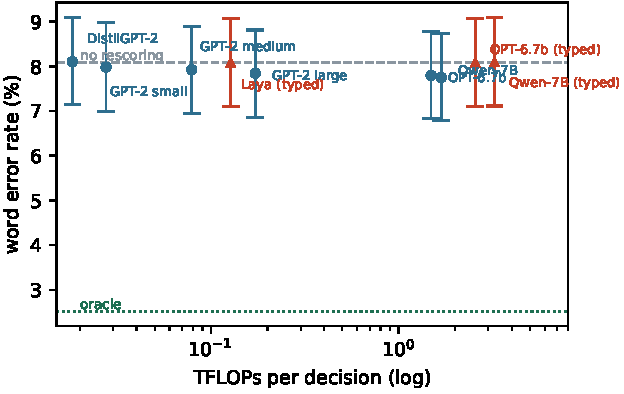
\includegraphics[width=0.68\linewidth]{fig_cost.pdf}
\caption{Word error against compute per decision (log scale). Circles are per-candidate
scoring, triangles typed selection, all at the published acoustic weight. The curve is
flat across two orders of magnitude of compute; re-tuning that weight
(Table~\ref{tab:joint}) tilts it in favour of the 7B models. Plotted points are the
exact Table~\ref{tab:main} values; the table rounds to one decimal.}
\label{fig:cost}
\end{figure}

At the published acoustic weight, rescoring is barely worth doing. The first pass alone scores
\werNone\% WER and the best open rescorer reaches \werOpt\%. Table~\ref{tab:main} and
Figure~\ref{fig:cost} sweep 82M to 7.6B parameters, and the per-candidate curve is flat
to within measurement noise. \textbf{DistilGPT-2 (\parDistil) lands exactly on the
baseline at \werDistil\%}, and the full 93$\times$ range buys three-tenths of a point.
The spread is smaller than the uncertainty on any single arm: every 95\% interval in
Table~\ref{tab:main} spans about two points and every interval overlaps every other, so
the marginal estimates alone cannot separate a 82M rescorer from a 7.6B one. The paired
bootstrap below is the sensitive test, because it holds the sentence sample fixed across
arms, and it does not separate them either.

\begin{table}[t]
\centering\small
\setlength{\tabcolsep}{4pt}
\begin{tabular}{lrlrr}
\toprule
Comparison (A vs.\ B) & $\Delta$WER & 95\% CI & $p$ & $p_{\text{Holm}}$ \\
\midrule
GPT-2 large (per-cand.) vs.\ OPT-6.7b & +0.05 & [-0.15, +0.24] & 0.701 & --- \\
Qwen2.5-7B (per-cand.) vs.\ OPT-6.7b & -0.05 & [-0.40, +0.30] & 0.413 & --- \\
Jev (hosted) (typed) vs.\ OPT-6.7b & -0.34 & [-0.80, +0.12] & 0.082 & --- \\
Jev (hosted) (typed) vs.\ GPT-2 large & -0.38 & [-0.85, +0.08] & 0.057 & --- \\
Laya (typed) vs.\ GPT-2 large & +0.25 & [-0.03, +0.53] & 0.963 & --- \\
OPT-6.7b (typed) vs.\ OPT-6.7b & +0.29 & [-0.02, +0.59] & 0.972 & --- \\
Qwen2.5-7B (typed) vs.\ Qwen2.5-7B & +0.35 & [-0.08, +0.77] & 0.949 & --- \\
Jev (hosted) (typed) vs.\ No rescoring (first pass only) & -0.63 & [-1.12, -0.14] & 0.006 & 0.042 \\
Qwen2.5-7B (per-cand.) vs.\ No rescoring (first pass only) & -0.34 & [-0.76, +0.09] & 0.064 & 0.256 \\
OPT-6.7b (per-cand.) vs.\ No rescoring (first pass only) & -0.29 & [-0.59, +0.02] & 0.035 & 0.21 \\
GPT-2 large (per-cand.) vs.\ No rescoring (first pass only) & -0.25 & [-0.53, +0.03] & 0.050 & 0.25 \\
GPT-2 medium (per-cand.) vs.\ No rescoring (first pass only) & -0.17 & [-0.40, +0.06] & 0.079 & 0.256 \\
GPT-2 small (per-cand.) vs.\ No rescoring (first pass only) & -0.11 & [-0.48, +0.25] & 0.315 & 0.63 \\
DistilGPT-2 (per-cand.) vs.\ No rescoring (first pass only) & +0.02 & [-0.23, +0.26] & 0.587 & 0.63 \\
OPT-6.7b (per-cand.) vs.\ GPT-2 small & -0.18 & [-0.48, +0.11] & 0.104 & --- \\
\bottomrule
\end{tabular}

\caption{Paired bootstrap on the test split, each arm at its tuned $\alpha$ and the
published acoustic weight.
$p_{\text{Holm}}$ is the Holm step-down correction over the seven arms-vs-baseline
comparisons; only Jev survives it.}
\label{tab:sig}
\end{table}

Table~\ref{tab:sig} gives explicit significance, and it disciplines the reading. Against
no rescoring, Jev ($-0.63$, $p=0.006$) is the only arm that survives Holm correction for
the seven arms tested (adjusted $p=0.042$); OPT-6.7b ($-0.29$, raw $p=0.035$) does not
(adjusted $p=0.21$), and neither do Qwen ($p=0.064$, adjusted $0.256$), GPT-2 large
($p=0.050$, adjusted $0.25$), or any smaller model (all adjusted $p \ge 0.25$). Within
open models, scale buys nothing measurable at this weight: OPT-6.7b against GPT-2 small is $-0.18$ at
$p=0.10$. That reading depends on holding the decoder's acoustic weight at its published
value, which was chosen for the decoder alone.

\paragraph{Re-tuning the decoder's weight.} Once a rescorer is added, the acoustic weight
is one more setting of the combined system, and nothing ties it to 0.3. We therefore tune
it jointly with $\alpha$ on the development split (acoustic weight over 17 values in
$[0, 5]$, $\alpha$ over 21 in $[0, 1]$), evaluate once on the test split, and compare
against no rescoring, whose own development-tuned weight is again 0.3
(Table~\ref{tab:joint}). The two 7B-class open models now separate clearly: OPT-6.7b
reaches \werOptJoint\% ($-0.89$, Holm-adjusted $p<0.001$) and Qwen2.5-7B \werQwenJoint\%
($-0.67$, adjusted $p=0.010$), while no model under 1B parameters does (all adjusted
$p \ge 0.27$). Scale now buys something: OPT-6.7b beats GPT-2 small by $0.70$ points
($p<0.001$). The optimum is broad rather than a lucky grid point: every setting within
0.05 of it in both weights lands between 7.20\% and 7.40\% on test. The closed typed arm
is best at \werJevJoint\%, with its tuned acoustic weight at 2.0, where it largely takes
over the $n$-gram's role, but it does not separate from OPT-6.7b ($-0.28$, 95\% CI
$[-0.72, +0.15]$, $p=0.11$). The revised reading is that the stage is worth under a
point once the decoder is strong, that only 7B-class models capture it, and that the
published fixed-weight protocol understates it by about two-thirds.

\begin{table}[t]
\centering\small
\setlength{\tabcolsep}{3pt}
\begin{tabular}{lrrrlrr}
\toprule
Arm & acoustic & $\alpha$ & WER & $\Delta$ vs.\ none [95\% CI] & $p$ & $p_{\text{Holm}}$ \\
\midrule
No rescoring & 0.30 & --- & 8.09 & --- & --- & --- \\
DistilGPT-2 (82M) & 0.35 & 0.35 & 8.15 & +0.06 [-0.31, +0.43] & 0.651 & 0.651 \\
GPT-2 small (124M) & 0.40 & 0.40 & 7.91 & -0.18 [-0.61, +0.26] & 0.222 & 0.444 \\
GPT-2 medium (355M) & 0.45 & 0.40 & 7.75 & -0.34 [-0.76, +0.10] & 0.067 & 0.268 \\
GPT-2 large (774M) & 0.50 & 0.45 & 7.77 & -0.32 [-0.83, +0.18] & 0.114 & 0.343 \\
OPT-6.7b & 0.40 & 0.45 & \textbf{7.20} & -0.89 [-1.35, -0.44] & $<$0.001 & $<$0.001 \\
Qwen2.5-7B & 0.45 & 0.45 & \textbf{7.42} & -0.67 [-1.15, -0.21] & 0.002 & 0.010 \\
Jev (hosted, typed) & 2.0 & 0.75 & \textbf{6.93} & -1.17 [-1.67, -0.68] & $<$0.001 & $<$0.001 \\
\midrule
Laya (typed) & 0.30 & 0.00 & 8.09 & 0.00 & --- & --- \\
OPT-6.7b (typed) & 0.25 & 0.20 & 8.37 & +0.28 [+0.11, +0.47] & --- & --- \\
Qwen2.5-7B (typed) & 0.30 & 0.20 & 8.11 & +0.02 [-0.22, +0.25] & --- & --- \\
\bottomrule
\end{tabular}

\caption{The decoder's acoustic weight re-tuned jointly with $\alpha$ per arm on the
development split; test split, paired bootstrap (5{,}000, one-sided) against no
rescoring; $p_{\text{Holm}}$ over the same seven arms as Table~\ref{tab:sig}. Bold: arms
that survive correction. Open typed arms (bottom) remain at or below the baseline.}
\label{tab:joint}
\end{table}

\paragraph{The gain depends on first-pass strength.} The same arms on our earlier weaker
first pass (\werNoneWeak\% WER, oracle \oracleWerWeak\%, truth in list \truthInListWeak\%)
told the opposite story: OPT-6.7b reached \werOptWeak\%, a 3.2-point gain, and DistilGPT-2
at \werDistilWeak\% captured about a third of it. Those two pipelines differ in decoder,
language model and menu size, so on their own they are an observed association rather than
a controlled comparison. We therefore vary first-pass strength directly: holding the
decoder and the candidate sets fixed, we sweep the acoustic scale from 0 to 1.0 and
re-rank. This moves first-pass error from \fpWeakSweep\% down to \werNone\% at the
published scale of 0.3, degrading again past it, with a single variable changed. It is a
rerank of fixed candidates, not a new beam decode.

Figure~\ref{fig:gaincollapse} shows the result for OPT-6.7b, with $\alpha$ re-tuned on
the development split at each scale. The gain is largest when the first pass is weak
(\gainWeak{} points at \fpWeakSweep\% WER) and shrinks to \gainStrong{} points at
\werNone\%. Past the published scale the gain grows again, partly because the first pass
degrades and partly because a heavier acoustic weight lets the rescorer take over the
$n$-gram's role: at 0.35 the first pass is unchanged at 8.09\% while OPT-6.7b reaches
7.43\%, and the joint optimum above adds \gainOptJoint{} points. Over the range a practitioner would operate in, the value of
rescoring is a decreasing function of first-pass strength, measured with one variable
changed. This is the paper's central result.

\begin{figure}[t]
\centering
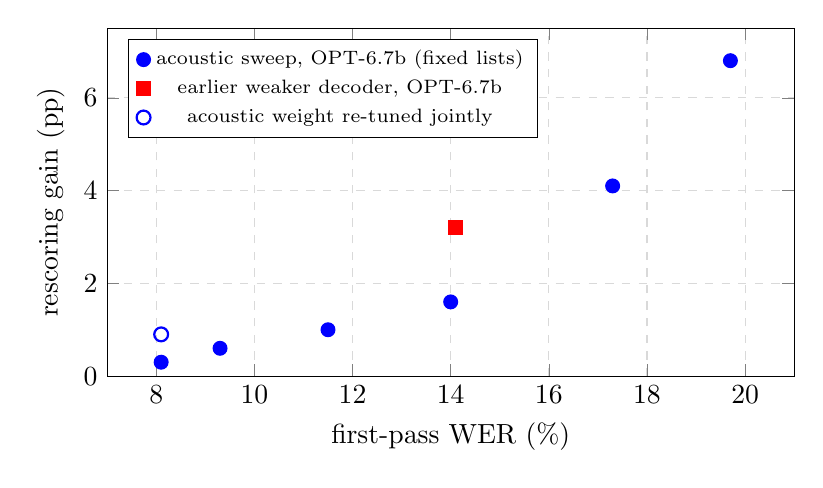
\begin{tikzpicture}
\begin{axis}[
  width=0.85\linewidth, height=6cm,
  xlabel={first-pass WER (\%)}, ylabel={rescoring gain (pp)},
  xmin=7, xmax=21, ymin=0, ymax=7.5,
  grid=major, grid style={dashed,gray!30},
  legend pos=north west, legend style={font=\scriptsize},
]
\addplot[only marks, mark=*, mark size=2.5pt, blue] coordinates {
(19.7,6.8) (17.3,4.1) (14.0,1.6) (11.5,1.0) (9.3,0.6) (8.1,0.3)
};
\addlegendentry{acoustic sweep, OPT-6.7b (fixed lists)}
\addplot[only marks, mark=square*, mark size=2.5pt, red] coordinates {(14.1,3.2)};
\addlegendentry{earlier weaker decoder, OPT-6.7b}
\addplot[only marks, mark=o, mark size=2.5pt, blue, thick] coordinates {(8.1,0.9)};
\addlegendentry{acoustic weight re-tuned jointly}
\end{axis}
\end{tikzpicture}
\caption{Rescoring gain collapses as first-pass strength increases. Blue points vary only the acoustic scale on fixed candidate sets;
the red square is the earlier weaker decoder (a different pipeline, shown separately).
Where the published decoder sits, at \werNone\% error, three-tenths of a point remain at
the published weight and \gainOptJoint{} with that weight re-tuned (hollow circle).}
\label{fig:gaincollapse}
\end{figure}

\paragraph{Error analysis: substitutions, and when overrides are right.} Errors are
dominated by substitutions: per 100 reference words the first pass makes \subsNone{}
substitutions, \insNone{} insertions and \delsNone{} deletions; OPT-6.7b moves those to
\subsOpt{}/\insOpt{}/\delsOpt{} and Jev to \subsJev{}/\insJev{}/\delsJev{}. Rescoring
trims substitutions and pays for part of it in insertions, but the bulk of the error
mass is untouched.

On the \nOverride{} test sentences where OPT-6.7b overrides the decoder's top
hypothesis, we relate the outcome to the decoder's own top-1/top-2 score margin.
Overrides of a confident decoder are the most likely to be right, 53\% correct in the
high-margin tercile against 26\% and 16\% in the low and middle, but with
point-biserial $r=\marginR$ the relationship is weak and non-monotonic, so margin does
not reliably predict an override's success. The predictable part of the gain sits exactly
where the truth is in the list: overrides cannot reach the truth on the 11\% of lists
where it is absent.

\section{The interpolation rule is not the bottleneck}
\label{sec:comb}

\begin{table}[t]
\centering\small
\begin{tabular}{lrrrr}
\toprule
Rescorer & V0 (z-norm) & V1 (raw+scale) & V2 (temperature) & V3 (MWER-lin.) \\
\midrule
OPT-6.7b & 7.80 & 7.71 & 7.71 & 7.83 \\
Qwen2.5-7B & 7.75 & 7.77 & 7.60 & 7.77 \\
GPT-2 large & 7.85 & 8.09 & 8.11 & 7.88 \\
GPT-2 medium & 7.92 & 8.03 & 8.09 & 7.89 \\
GPT-2 small & 7.98 & 8.12 & 8.37 & 8.03 \\
DistilGPT-2 & 8.11 & 8.06 & 8.50 & 8.03 \\
\bottomrule
\end{tabular}

\caption{Test WER for four score-combination schemes on identical lists, each tuned per
arm on the development split. No variant beats V0 once the 18 arm--variant comparisons
are accounted for (paired bootstrap, one-sided; best raw $p=0.019$ for DistilGPT-2 under
V3, Holm-adjusted $p=0.33$). V3 is a linear MWER-style fit of the two
scores, not a trained reranker.}
\label{tab:comb}
\end{table}

The efficiency curve could in principle be an artefact of how we combine scores. We test
that on the same cached lists with four variants, each tuned per arm on the development
split and evaluated on the disjoint test split: \textbf{V0}, the paper's rule ($z$-normalise
both scores per list, combine with weight $\alpha$); \textbf{V1}, raw length-normalised
log-likelihood with a learned global scale; \textbf{V2}, per-arm temperature scaling with
no extra weight; and \textbf{V3}, a discriminative MWER-style fit of the two scores on the
development split. V3 is a two-parameter interpolation, not a trained reranker: no encoder
is fine-tuned, so it is not comparable to RescoreBERT~\cite{rescorebert}.

No variant changes the picture (Table~\ref{tab:comb}). All four sit within noise on every
arm, and none beats V0 significantly once the 18 arm--variant comparisons are accounted
for (smallest raw $p=0.019$, Holm-adjusted $0.33$). Temperature scaling actively hurts the
two smallest arms (GPT-2 small $7.98 \rightarrow 8.37$, DistilGPT-2 $8.11 \rightarrow
8.50$), a reminder that dev-fitted combination can overfit on \nDev{} sentences. The
ranking of arms is invariant to the rule. None of these variants, however, touches the
decoder's own acoustic weight, and \S\ref{sec:efficiency} shows that weight matters more
than any of them.

A joint linear reranker over the first-pass score and five per-candidate arms, fit with
the same objective, reaches \mwerMulti\% against \werOpt\% for the best single arm
(paired $p=\mwerMultiP$), keeping OPT-6.7b and Qwen2.5-7B and zeroing the rest. It takes
the first-pass score as one fixed feature, so it cannot re-weight acoustic against
$n$-gram evidence; the joint re-tuning in \S\ref{sec:efficiency} can, and gains more.

\paragraph{Discriminative fine-tuning of the small rescorer.} The fits above move
scalars, not the model. The stronger test fine-tunes GPT-2 small itself with the MWER
objective on the cached lists: each training list contributes its top-20 candidates,
their length-normalised log-likelihoods become a posterior over the list, and the loss
is the expected word-error count under that posterior, backpropagated through the full
model. We train on 300 of the \nDev{} development lists (119 held out for early
stopping), AdamW at $10^{-5}$, batches of 4 lists, 3 epochs on an L40S; the
interpolation weight $\alpha$ is re-tuned on the development split and the final model
is evaluated on the disjoint \nTest{}-sentence test split, which was used for neither
training, early stopping, nor $\alpha$ selection. The pipeline reproduces both cached
baselines exactly before training (frozen GPT-2 small at $\alpha=0.4$: \werGptSmall\%;
no rescoring: \werNone\%). Held-out expected error falls from 0.201 to 0.195 across the
three epochs, so the objective learns, but the test result is \mwerSmallWer\% WER at
$\alpha=\mwerSmallAlpha$, against \werGptSmall\% frozen and \werNone\% for doing
nothing (paired bootstrap, one-sided: $p=\mwerSmallPNone$ vs.\ no rescoring,
$p=\mwerSmallPGpt$ vs.\ frozen GPT-2 small). Three epochs of discriminative training on
300 lists do not separate the small rescorer from the baseline by a measurable margin.
That is one recipe on one model: it shows this fine-tuning did not recover the headroom,
not that discriminative fine-tuning cannot.

\section{Listwise typed selection fails, and why}
\label{sec:typed}

\begin{table}[t]
\centering\small
\begin{tabular}{lrrrr}
\toprule
Typed rescorer & Labels used & Mass on A & Truth sel. & Truth sel.\ ($\ne$A) \\
\midrule
Jev (hosted) & 57 / 100 & 72\% & 67.9\% & 26.6\% \\
Laya & 44 / 100 & 69\% & 53.7\% & 2.3\% \\
OPT-6.7b & 13 / 100 & 35\% & 27.3\% & 0.2\% \\
Qwen2.5-7B & 31 / 100 & 28\% & 29.3\% & 2.4\% \\
\midrule
\emph{Top-1, no rescorer} & --- & --- & \emph{68.0\%} & --- \\
\bottomrule
\end{tabular}

\caption{Diagnostic for the typed arms over all \nLists{} lists (100-best generation; mean
38.7 candidates per list). ``Labels used'' counts distinct candidate labels ever selected;
``truth selected'' is how often the arm's own argmax is correct, before combination. Label
A is the decoder's top candidate. The last column conditions on deviating from it: only
Jev's deviations carry signal.}
\label{tab:collapse}
\end{table}

If the rescorer's job is to pick one of $N$ written-down options, an obvious efficiency
move is to ask for exactly that. It does not work for general language models: the two
open typed arms land on the no-rescoring baseline (Table~\ref{tab:main}), with OPT-6.7b
and Laya both tuning to $\alpha=0$, meaning the combination discards them entirely, and
only the closed Jev arm improves on it. Re-tuning the acoustic weight does not rescue the
open typed arms (Table~\ref{tab:joint}), while Jev becomes the strongest arm overall.

Table~\ref{tab:collapse} shows the mechanism, reproduced under the strong first pass.
Candidates are serialised in the decoder's ranking order, so label A is the decoder's own
top hypothesis, and all four typed arms collapse onto it, placing 28--72\% of their
decisions on that one label while using only 13--57 distinct labels across all lists. This
is the domain-specific form of the positional prior documented
by~\cite{tang2023psc,bito2026position}. What separates the arms is not the prior but the
deviations from it. Conditional on picking any label other than A, Jev selects the truth
27\% of the time; Laya, OPT-6.7b and Qwen2.5-7B manage 2\%, 0\% and 2\%. Only Jev's
deviations carry signal. Three arms are therefore a strong
prior over the first position plus noise; Jev is a strong prior over the first position
plus informative corrections, which is why it alone beats taking the decoder's top
hypothesis (\firstPassTopOne\% sentence accuracy) and doing nothing.

The prompt asks for the ``most fluent, natural English sentence,'' which could bias
selections toward fluency over correctness. It does not appear to. Using the cached per-candidate GPT-2 log-likelihoods as a fluency
proxy, Jev picks the most fluent candidate on 40.7\% of test lists but the truth on
77.6\%. Conditional on deviating from label A with the truth present, it picks the truth
40.2\% of the time against 24.7\% for the most fluent candidate. On the sharp subset
where truth and fluency disagree and Jev deviates ($N=144$), it picks the
true-but-less-fluent candidate 31.9\% of the time and the fluent-but-wrong one 19.4\%,
with 48.6\% going to neither. Its deviations lean
toward the true transcript \emph{despite} the fluency wording, not because of it:
though with $N=144$ a mild fluency lean cannot be ruled out. Label A is the fluency
argmax on only 35.6\% of lists, so position and fluency are entangled at the top but
not identified with each other.

\subsection{Menu size and permutation aggregation}
\label{sec:ablation}

\begin{table}[t]
\centering\small
\begin{tabular}{lrrrr}
\toprule
Menu size $N$ & 5 & 10 & 20 & 60 \\
\midrule
Truth available in menu & 56.5\% & 60.5\% & 64.5\% & 66.8\% \\
\midrule
Qwen2.5-7B (typed) & 76.1\% & 69.1\% & 59.2\% & 1.5\% \\
OPT-6.7b (typed) & 22.1\% & 40.0\% & 52.4\% & 55.1\% \\
\emph{Take first-pass top-1} & \emph{80.5\%} & \emph{75.2\%} & \emph{70.5\%} & \emph{68.2\%} \\
\midrule
\multicolumn{5}{l}{\emph{Permutation mitigation at $N=60$ (Borda over 5 shuffles)}} \\
\quad Qwen2.5-7B & \multicolumn{2}{r}{single order 1.5\%} & \multicolumn{2}{r}{Borda-5 56.9\%} \\
\quad OPT-6.7b & \multicolumn{2}{r}{single order 55.1\%} & \multicolumn{2}{r}{Borda-5 2.7\%} \\
\bottomrule
\end{tabular}

\caption{Accuracy \emph{conditional on the truth being present in the menu}, which differs
by $N$ and must be divided out. The italic row is the do-nothing baseline: take the
decoder's top hypothesis. Subset of 400 sentences. No configuration beats the decoder's
top hypothesis; permutation self-consistency rescues Qwen while destroying OPT.}
\label{tab:ablation}
\end{table}

Two obvious objections are that the menu is too long and that the prompt order is
arbitrary. We test both on the weaker-regime 60-best lists, where the typed arms' failure
was first characterised; the mechanism finding carries over to the published regime above.
Because shorter menus contain the truth less often (from \ldots\ 56.5\% at $N=5$ to 66.8\%
at $N=60$), raw selection accuracy is not comparable across $N$.
Table~\ref{tab:ablation} therefore reports accuracy conditional on the truth being available.

The two failures separate cleanly. \textbf{Qwen2.5-7B is menu-length sensitive}: it reaches
\qwenTypedAtFive\% at $N=5$, using every available label, and degrades monotonically to
\qwenTypedAtSixty\% at $N=60$. \textbf{OPT-6.7b is not}: it uses three of five labels even
at $N=5$ and never approaches the baseline. Applying permutation self-consistency
(Borda over five shuffles) at $N=60$ separates them further: it \emph{rescues} Qwen
(\qwenTypedAtSixty\% $\rightarrow$ \qwenBorda\%, roughly its $N=20$ level) and
\emph{destroys} OPT (\optTypedAtSixty\% $\rightarrow$ \optBorda\%). This is what one
should expect: aggregation recovers signal that order noise obscured, but a model with a
fixed positional prior has no candidate-dependent signal to aggregate, so shuffling
converts its answer into noise. The mitigation therefore doubles as a diagnostic for which
failure mode is present.

Neither repair is sufficient. Qwen's best configuration (\qwenTypedAtFive\% at $N=5$)
remains below the \baseAtFive\% obtained by taking the decoder's top hypothesis, and its
rescued $N=60$ result (\qwenBorda\%) remains below \baseAtSixty\%. \emph{No general
language model we tested performs listwise typed selection well enough to be worth running
at all.}

\section{Where the gains live, and abstention}
\label{sec:abstain}

\begin{table}[t]
\centering\small
\begin{tabular}{lrrrrrr}
\toprule
 & \multicolumn{3}{c}{Truth in list (\nInList{} sent.)} & \multicolumn{3}{c}{Truth absent (\nOutList{} sent.)} \\
\cmidrule(lr){2-4}\cmidrule(lr){5-7}
Arm & WER & $\Delta$ vs none & $p$ & WER & $\Delta$ vs none & $p$ \\
\midrule
No rescoring & 4.37 & --- & --- & 36.56 & --- & --- \\
OPT-6.7b & 4.05 & -0.31 & 0.035 & 36.42 & -0.13 & 0.433 \\
Qwen2.5-7B & 4.04 & -0.33 & 0.077 & 36.16 & -0.40 & 0.342 \\
GPT-2 small & 4.28 & -0.09 & 0.346 & 36.29 & -0.27 & 0.360 \\
Jev (typed) & 3.80 & -0.57 & 0.015 & 35.50 & -1.06 & 0.123 \\
\bottomrule
\end{tabular}

\caption{Test WER split by whether the reference transcript is in the candidate list.
Gains concentrate where the truth is present; where it is absent, no arm moves the needle.
Paired bootstrap vs.\ no rescoring within each group.}
\label{tab:truth}
\end{table}

\begin{table}[t]
\centering\small
\begin{tabular}{llrrrrrr}
\toprule
 & & & \multicolumn{5}{c}{sentence error among spoken, at coverage} \\
\cmidrule(lr){4-8}
Rescorer & Shape & ECE & 30\% & 50\% & 70\% & 90\% & 100\% \\
\midrule
\bf Jev (hosted) & typed & 0.088 & \bf 3\% & \bf 8\% & \bf 13\% & \bf 22\% & \bf 29\% \\
Laya & typed & 0.324 & 9\% & 10\% & 19\% & 28\% & 30\% \\
OPT-6.7b & typed & 0.220 & 9\% & 13\% & 21\% & 27\% & 30\% \\
Qwen2.5-7B & typed & 0.095 & 9\% & 16\% & 21\% & 25\% & 30\% \\
OPT-6.7b & per-cand.\ + softmax & 0.160 & 8\% & 10\% & 17\% & 24\% & 28\% \\
GPT-2 large & per-cand.\ + softmax & 0.136 & 9\% & 13\% & 18\% & 25\% & 29\% \\
Qwen2.5-7B & per-cand.\ + softmax & 0.116 & 9\% & 15\% & 18\% & 25\% & 29\% \\
\bottomrule
\end{tabular}

\caption{Coverage--risk. Per-candidate arms receive a temperature-calibrated softmax over
their candidate scores, temperature fit on the development split, so they are not
disadvantaged merely by lacking a native probability.}
\label{tab:abstention}
\end{table}

The reference transcript is absent from the candidate list on $100-\truthInList = 11\%$ of
sentences, and there no rescorer can succeed. Splitting the test set on that boundary
(\nInList{} vs.\ \nOutList{} sentences) locates the entire effect: OPT-6.7b improves
in-list WER by \optInListDelta{} points ($p=\optInListP$) and Jev by \jevInListDelta{}
($p=\jevInListP$), while out-of-list WER barely moves for any arm (Table~\ref{tab:truth}).

This bounds what abstention can buy. Selecting the 50\% most confident sentences
\emph{within each group}, sentence error is 100\% whenever the truth is absent, for the
typed arm and for the calibrated per-candidate baseline alike: there is nothing to select.
Abstention helps only by declining sentences no rescorer could have fixed.

A fair comparison requires giving per-candidate arms a confidence, which they lack
natively; we fit a softmax temperature on the development split. That baseline has teeth
(Table~\ref{tab:abstention}): OPT falls from \riskOptAtHundred\% error at full coverage to
\riskOptAtThirty\% at 30\%. Jev's curve is the strongest (\riskJevAtHundred\% to
\riskJevAtThirty\%), but the gap is one of degree, and of \emph{ranking} rather than
calibration. Isotonic recalibration introduces zero rank inversions and leaves the curve
unchanged, and the max softmax probability already beats the top-1/top-2 margin among
per-candidate signals. At full coverage OPT and Jev have the same sentence error (28.4\%
vs.\ 28.7\%); Jev's curve falls faster because its confidences separate right from wrong
decisions more sharply (0.736 vs.\ 0.409, against OPT's 0.647 vs.\ 0.368). This is one
closed model, not a property of typed decisions.

\paragraph{Candidate-set size.} Pruning to the decoder's top 20 raises the oracle from
2.5\% to 3.3\% and drops truth-in-list from 89\% to 86\%, bounding what any selection
method could reach. The efficiency conclusion survives: with $\alpha$ retuned on pruned
development lists, Qwen2.5-7B and GPT-2 large remain significant ($p=0.024$, $p=0.045$),
OPT slips below the bar ($p=0.12$), and the 93$\times$ parameter spread is 0.4pp at
$N=20$ against 0.3pp at $N=100$.

\section{Limitations}

\begin{itemize}\itemsep2pt
\item \textbf{One participant, one split, limited power.} T15, \texttt{val}, \nTest{} test
  sentences. Effects here are under a point and bootstrap intervals span roughly
  a point, so the study detects effects around half a point and above. Read ``no
  improvement'' as ``none large enough for this sample to see.'' No other T15 session with
  released transcripts was available, so cross-session generalisation is untested.
\item \textbf{Text-only, untuned, no earlier fusion.} No arm conditions on acoustics or is
  fused before the second pass, so the curve does not bound what acoustic access could
  achieve~\cite{kim2022joint}. On discriminative fine-tuning we have one test
  (\S\ref{sec:comb}): one model, one objective, 300 training lists. A larger effort could
  still shift the curve.
\item \textbf{Results depend on the protocol.} Holding the decoder's acoustic weight at
  its published value, as our main tables do, understates the stage by about two-thirds;
  we report both protocols. The joint search over two weights is fit on \nDev{} sentences.
\item \textbf{The first-pass sweep reranks fixed candidate sets.} Varying the acoustic
  scale changes first-pass strength without re-running the beam decode, so the candidate
  pool is fixed by construction.
\item \textbf{Typed failures are not exhaustive.} Four models, one prompt template
  (Appendix~\ref{app:prompt}), one label construction, one aggregation scheme. The
  instruction asks for the ``most fluent, natural English sentence,'' which may bias
  selection toward fluency over correctness; we quantify that confound in
  \S\ref{sec:typed} but did not test alternative wordings. The menu-size and Borda
  ablations use the earlier 60-best lists; the collapse itself is confirmed on the
  published lists in Table~\ref{tab:collapse}.
\item \textbf{One typed arm is closed}, so both the working listwise result and the
  abstention observation rest on a model a reader cannot inspect. We release its cached
  lists, prompt template, label mappings, per-sentence label probabilities and the
  $\alpha$ settings, so the analysis is reproducible even though the model is not.
\end{itemize}

\section{Conclusion}

On real intracortical recordings with the published decoder, the language-model rescoring
stage contributes under a word-error point. At the published acoustic weight, a 93$\times$
range of model size moves word error three-tenths of a point and no open model clears
significance after Holm correction. Re-tuning that weight with the rescorer roughly triples
the gain for the 7B-class open models (\werNone\% $\rightarrow$ \werOptJoint\% for
OPT-6.7b), which then separate from both the baseline and the small models; nothing under
1B parameters does under either protocol. The strongest arm under both is closed
(Jev~\cite{typesafe2026jev}) and does not separate from OPT-6.7b; we read it as evidence
that a purpose-built typed model can do the job, not as a deployable or cost result.

Collapsing the stage into a single listwise typed decision does not work for general
language models. Every typed arm piles most of its decisions on the decoder's top
candidate, and only Jev's deviations from that prior carry signal. Permutation
self-consistency rescues one failure mode while destroying the other, without making
either competitive with doing nothing.

The stage mattered when the first pass was weaker. On our earlier \werNoneWeak\%-error
decoder it was worth 3.2 points, and a controlled sweep varying only the acoustic scale
puts the gain at \gainWeak{} points at \fpWeakSweep\% first-pass WER against
\gainStrong--\gainOptJoint{} at \werNone\%, depending on whether the acoustic weight is
re-tuned. Four interpolation schemes, a jointly fit reranker and a discriminatively
fine-tuned GPT-2 small all land within noise; the one setting that matters is the
decoder's own weight, and even with it re-tuned the gain at a strong first pass is a
fraction of the gain at a weak one.

One hypothesis fits the remaining puzzle. Oracle WER is \oracleWer\% against \werNone\%
first-pass, yet text-only models exploit almost none of that headroom. A plausible
explanation is that the errors a strong first pass leaves are increasingly acoustically
ambiguous rather than resolvable from candidate text alone. Our data cannot settle this,
since every arm here is text-only; an acoustically conditioned rescorer on the same lists
would.

\appendix

\section{Prompt template, serialisation and label alphabet}
\label{app:prompt}

Typed arms receive one prompt per list. Candidates are serialised one per line as
\texttt{<label>: <sentence>}, in the decoder's own ranking order unless stated otherwise,
with the instruction block held fixed:

\begin{quote}\small\ttfamily
A speech decoder produced these candidate sentences for what a person was\\
trying to say. Exactly one is what they meant.\\
Answer with the single label of the
most fluent, natural English sentence.\\[2pt]
A: <candidate 1>\\
B: <candidate 2>\\
\ldots\\[2pt]
Answer:
\end{quote}

For chat-tuned models the block is wrapped in the model's own chat template and the
assistant turn is opened with the scaffold \texttt{"The answer is "}, so that the first free
token position coincides with the label. Labels are built greedily from
\texttt{A}--\texttt{Z}, then decimal numerals, then \texttt{a}--\texttt{z}, then two-letter
combinations \texttt{AA}--\texttt{ZZ} (the extension was needed for 100-option menus: some
tokenizers yield only 61 single-token labels from the shorter pool), keeping a
candidate only if it encodes to exactly one token in that model's vocabulary and its id has
not already been used; duplicates are skipped rather than reused, so the map from label to
candidate is injective. Scores are read as the model's log-probability at the single answer
position, restricted to the label token ids and renormalised over the menu.

\section{Token accounting}
\label{app:tokens}

Per-candidate arms read every candidate once: at a mean of 38.7 candidates per list and
32.2 characters each, \tokPerCand{} tokens per decision at $\approx$4 characters/token.
Typed arms read the same candidates plus labels and instructions in one prompt, a measured
median of \tokTypedOpt{} tokens (OPT tokenizer) and \tokTypedQwen{} (Qwen). The two
shapes read comparable amounts of text, so the compute difference in Table~\ref{tab:main}
follows model size, not the number of forward passes. FLOPs are
$2 \times \text{params} \times \text{tokens}$, ignoring attention's quadratic term,
which is negligible at these lengths.

\begin{thebibliography}{9}\small

\bibitem{willett2023}
F.~R. Willett et al.
\newblock A high-performance speech neuroprosthesis.
\newblock \emph{Nature}, 620:1031--1036, 2023.

\bibitem{b2tbench}
Brain-to-Text Benchmark reference implementation and T15 dataset.
\newblock \url{https://github.com/Neuroprosthetics-Lab/nejm-brain-to-text}.

\bibitem{zhang2022opt}
S.~Zhang et al.
\newblock OPT: Open pre-trained transformer language models.
\newblock arXiv:2205.01068, 2022.

\bibitem{graves2006ctc}
A.~Graves, S.~Fern\'andez, F.~Gomez, and J.~Schmidhuber.
\newblock Connectionist temporal classification: labelling unsegmented sequence data with
  recurrent neural networks.
\newblock In \emph{ICML}, 2006.

\bibitem{rescorebert}
L.~Xu, Y.~Gu, J.~Kolehmainen, H.~Khan, A.~Gandhe, A.~Rastrow, A.~Stolcke, and I.~Bulyko.
\newblock RescoreBERT: Discriminative speech recognition rescoring with BERT.
\newblock In \emph{ICASSP}, 2022. arXiv:2202.01094.

\bibitem{tang2023psc}
R.~Tang, X.~Zhang, X.~Ma, J.~Lin, and F.~Ture.
\newblock Found in the middle: permutation self-consistency improves listwise ranking in
  large language models.
\newblock In \emph{NAACL}, 2024. arXiv:2310.07712.

\bibitem{bito2026position}
E.~Bito, Y.~Ren, and E.~He.
\newblock Position bias undermines preference consistency in listwise LLM-based reranking.
\newblock arXiv:2608.03091, 2026.

\bibitem{lob2023}
Y.~Yu, C.-H.~H.~Yang, J.~Kolehmainen, P.~G.~Shivakumar, Y.~Gu, S.~Ryu, R.~Ren,
Q.~Luo, A.~Gourav, I.-F.~Chen, Y.-C.~Liu, T.~Dinh, A.~Gandhe, D.~Filimonov,
S.~Ghosh, A.~Stolcke, A.~Rastrow, and I.~Bulyko.
\newblock Low-rank adaptation of large language model rescoring for
  parameter-efficient speech recognition.
\newblock In \emph{ASRU}, 2023. arXiv:2309.15223.

\bibitem{shivakumar2023disc}
P.~G.~Shivakumar, J.~Kolehmainen, Y.~Gu, A.~Gandhe, A.~Rastrow, and I.~Bulyko.
\newblock Discriminative speech recognition rescoring with pre-trained language
  models.
\newblock In \emph{ASRU}, 2023. arXiv:2310.06248.

\bibitem{udagawa2022}
T.~Udagawa, M.~Suzuki, G.~Kurata, N.~Itoh, and G.~Saon.
\newblock Effect and analysis of large-scale language model rescoring on competitive ASR
  systems.
\newblock In \emph{Interspeech}, 2022. arXiv:2204.00212.

\bibitem{yang2023generative}
C.-H.~H.~Yang, Y.~Gu, Y.-C.~Liu, S.~Ghosh, and I.~Bulyko.
\newblock Generative speech recognition error correction with large language models and
  task-activating prompting.
\newblock arXiv:2309.15649, 2023.

\bibitem{shivakumar2024speechtext}
P.~G.~Shivakumar, J.~Kolehmainen, A.~Gourav, Y.~Gu, and A.~Gandhe.
\newblock Speech recognition rescoring with large speech-text foundation models.
\newblock arXiv:2409.16654, 2024.

\bibitem{chen2023longform}
T.~Chen, C.~Allauzen, Y.~Huang, D.~Park, D.~Rybach, and W.~R.~Huang.
\newblock Large-scale language model rescoring on long-form data.
\newblock arXiv:2306.08133, 2023.

\bibitem{kim2022joint}
S.~Kim, K.~Li, L.~Kabela, R.~Huang, J.~Zhu, O.~Kalinli, and D.~Le.
\newblock Joint audio/text training for transformer rescorer of streaming speech
  recognition.
\newblock In \emph{Findings of EMNLP}, 2022.

\bibitem{bito2026invarirank}
E.~Bito, Y.~Ren, and E.~He.
\newblock One pass, any order: position-invariant listwise reranking for LLM-based
  recommendation.
\newblock arXiv:2604.27599, 2026.

\bibitem{radford2019gpt2}
A.~Radford, J.~Wu, R.~Child, D.~Luan, D.~Amodei, and I.~Sutskever.
\newblock Language models are unsupervised multitask learners.
\newblock OpenAI technical report, 2019.

\bibitem{typesafe2026jev}
T.~Claburn.
\newblock TypeSafe AI debuts model for machines that plays Doom.
\newblock \emph{The Register}, 16 Sep 2026.
\newblock \url{https://www.theregister.com/ai-and-ml/2026/09/16/typesafe-ai-debuts-model-for-machines-that-plays-doom/5296711}.

\end{thebibliography}

\end{document}
